This chapter provides a high-level overview of the core components of the AirSim architecture. The chapter will look at how the simulator has been adapted for this project, the design decisions made, and the limitations. 

As the project is extending an existing code-base, the design decisions aimed to limit the impact on the existing structure. This was to allow future updates to the master project, to benefit this one as well. Most of the changes to this project were made in Unity, but changes were also made in AirLib and the wrapper to allow for additional APIs. 

\section{AirSim Functional Overview}
Figure~\ref{ADA:Figure:OriginalOverview} shows a simplified overview of the important components in the original AirSim architecture. It is key to understand each of these components, as they are all updated throughout the project. 


The project consists of 4 main components, Unity, which is written in C\# and contains most of the simulator logic, AirLib which is written in C++ and contains the server, the AirLib Wrapper which is written in C++ and acts as a bridge between AirLib and Unity, then finally the code where the user can interact with AirLib through the APIs. As this project is very modular, it gives the user the freedom and flexibility to choose a game engine and input language. 

\subsection{User Interaction Layer}

\subsection{AirLib}

\subsection{AirLib Wrapper}

\subsection{AirSim with Unity}

\begin{figure}[H]
    \centering
    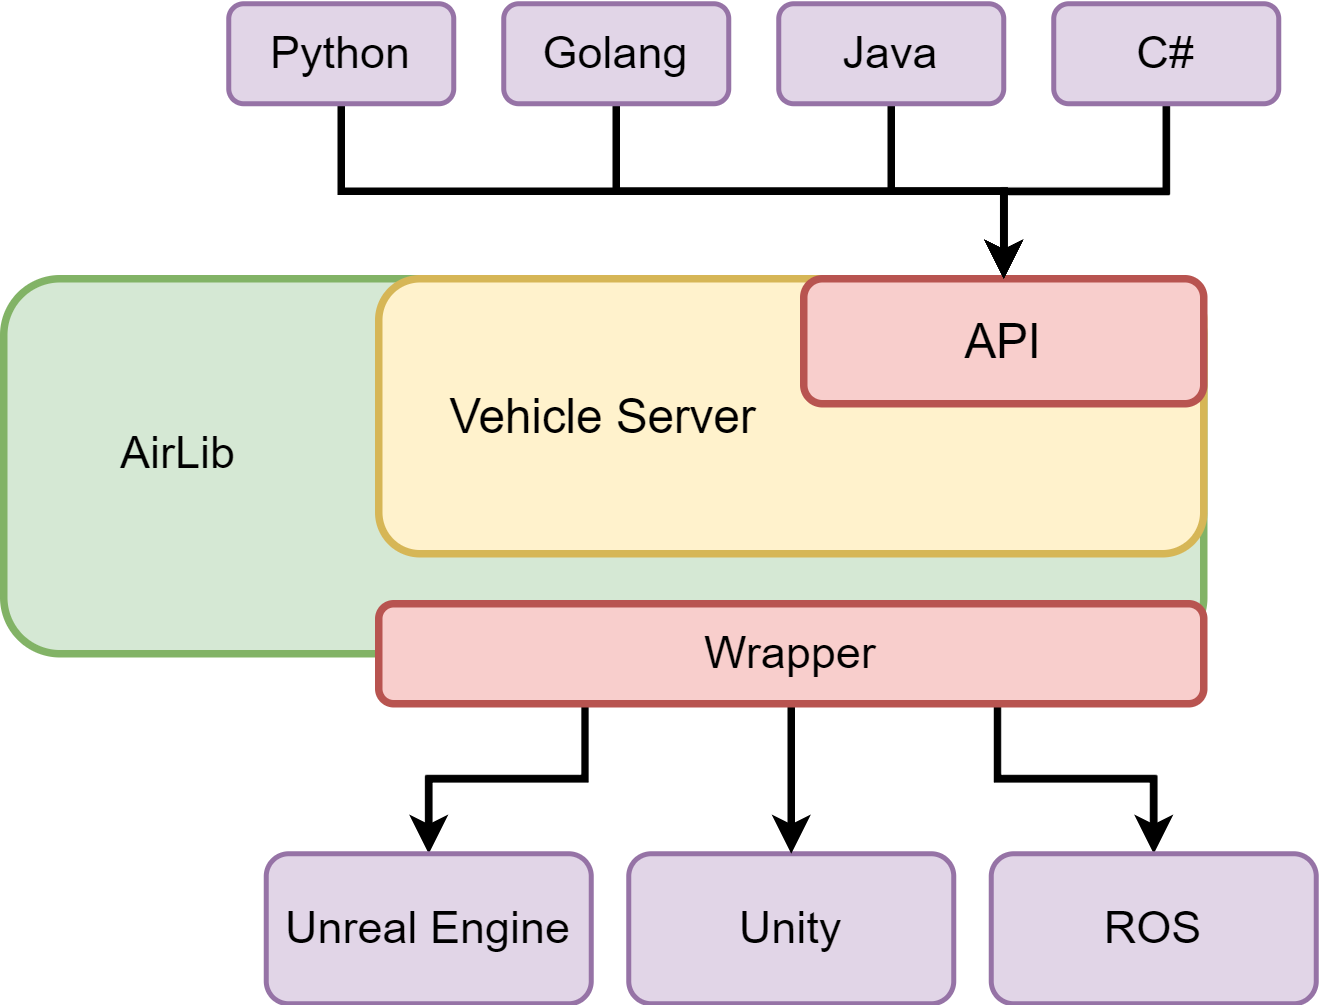
\includegraphics[width=0.7\textwidth]{05_AnalysisAndDesign/Diagrams/OriginalOverview.png}
    \caption{High-level overview of the core components of AirSim used for this project. Only one server exists.}
    \label{ADA:Figure:OriginalOverview}
    
\end{figure}

\begin{figure}[H]
    \centering
    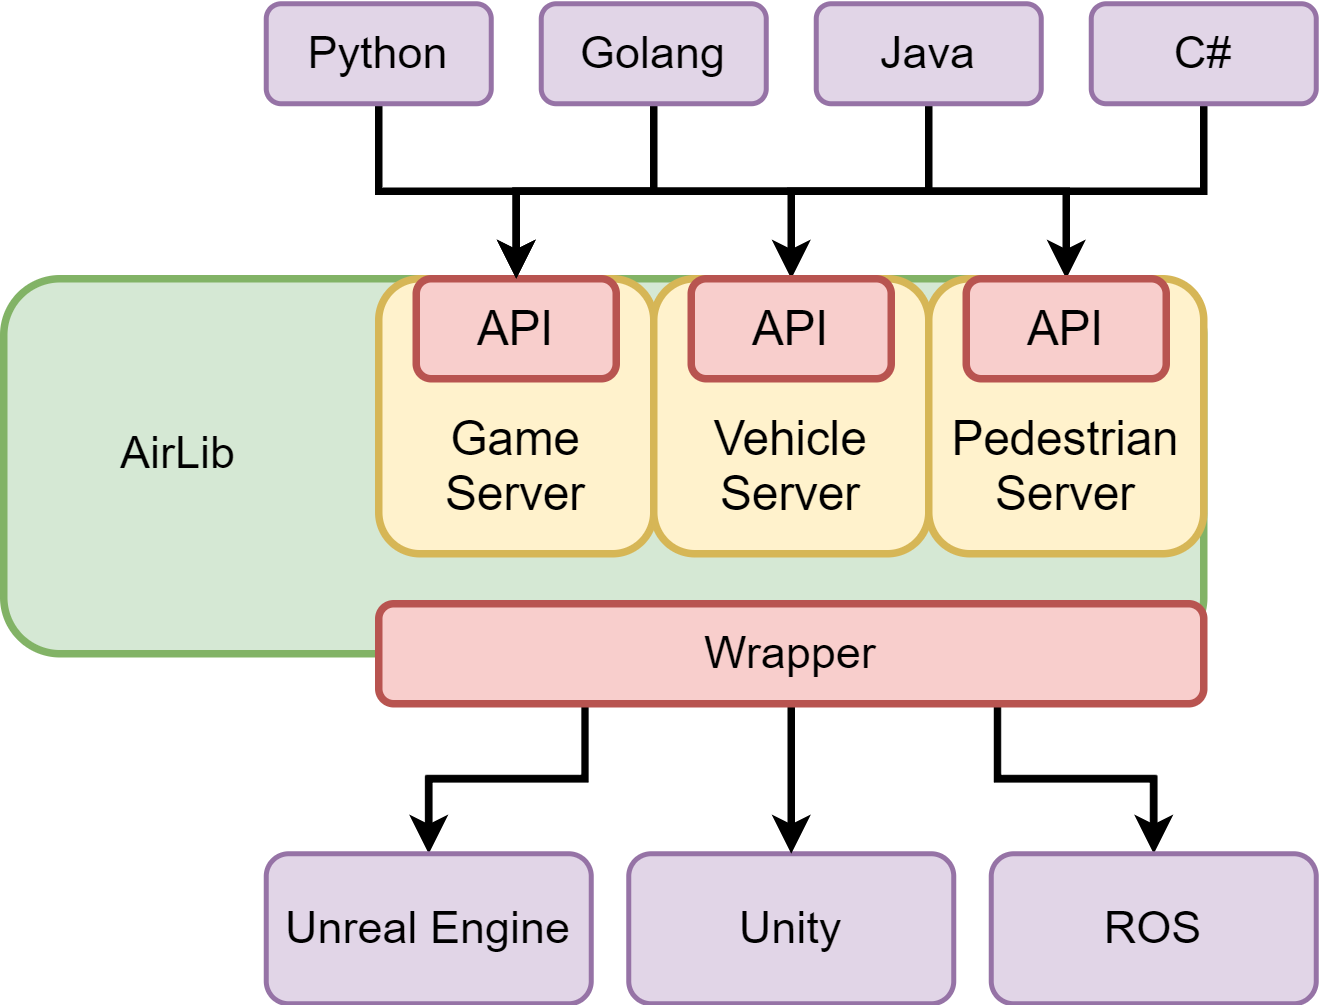
\includegraphics[width=0.7\textwidth]{05_AnalysisAndDesign/Diagrams/UpdatedOverview.png}
    \caption{Separate APIs into several servers on different ports. This makes it easier to expand the APIs and add additional features}
\end{figure}

\begin{figure}[H]
    \centering
    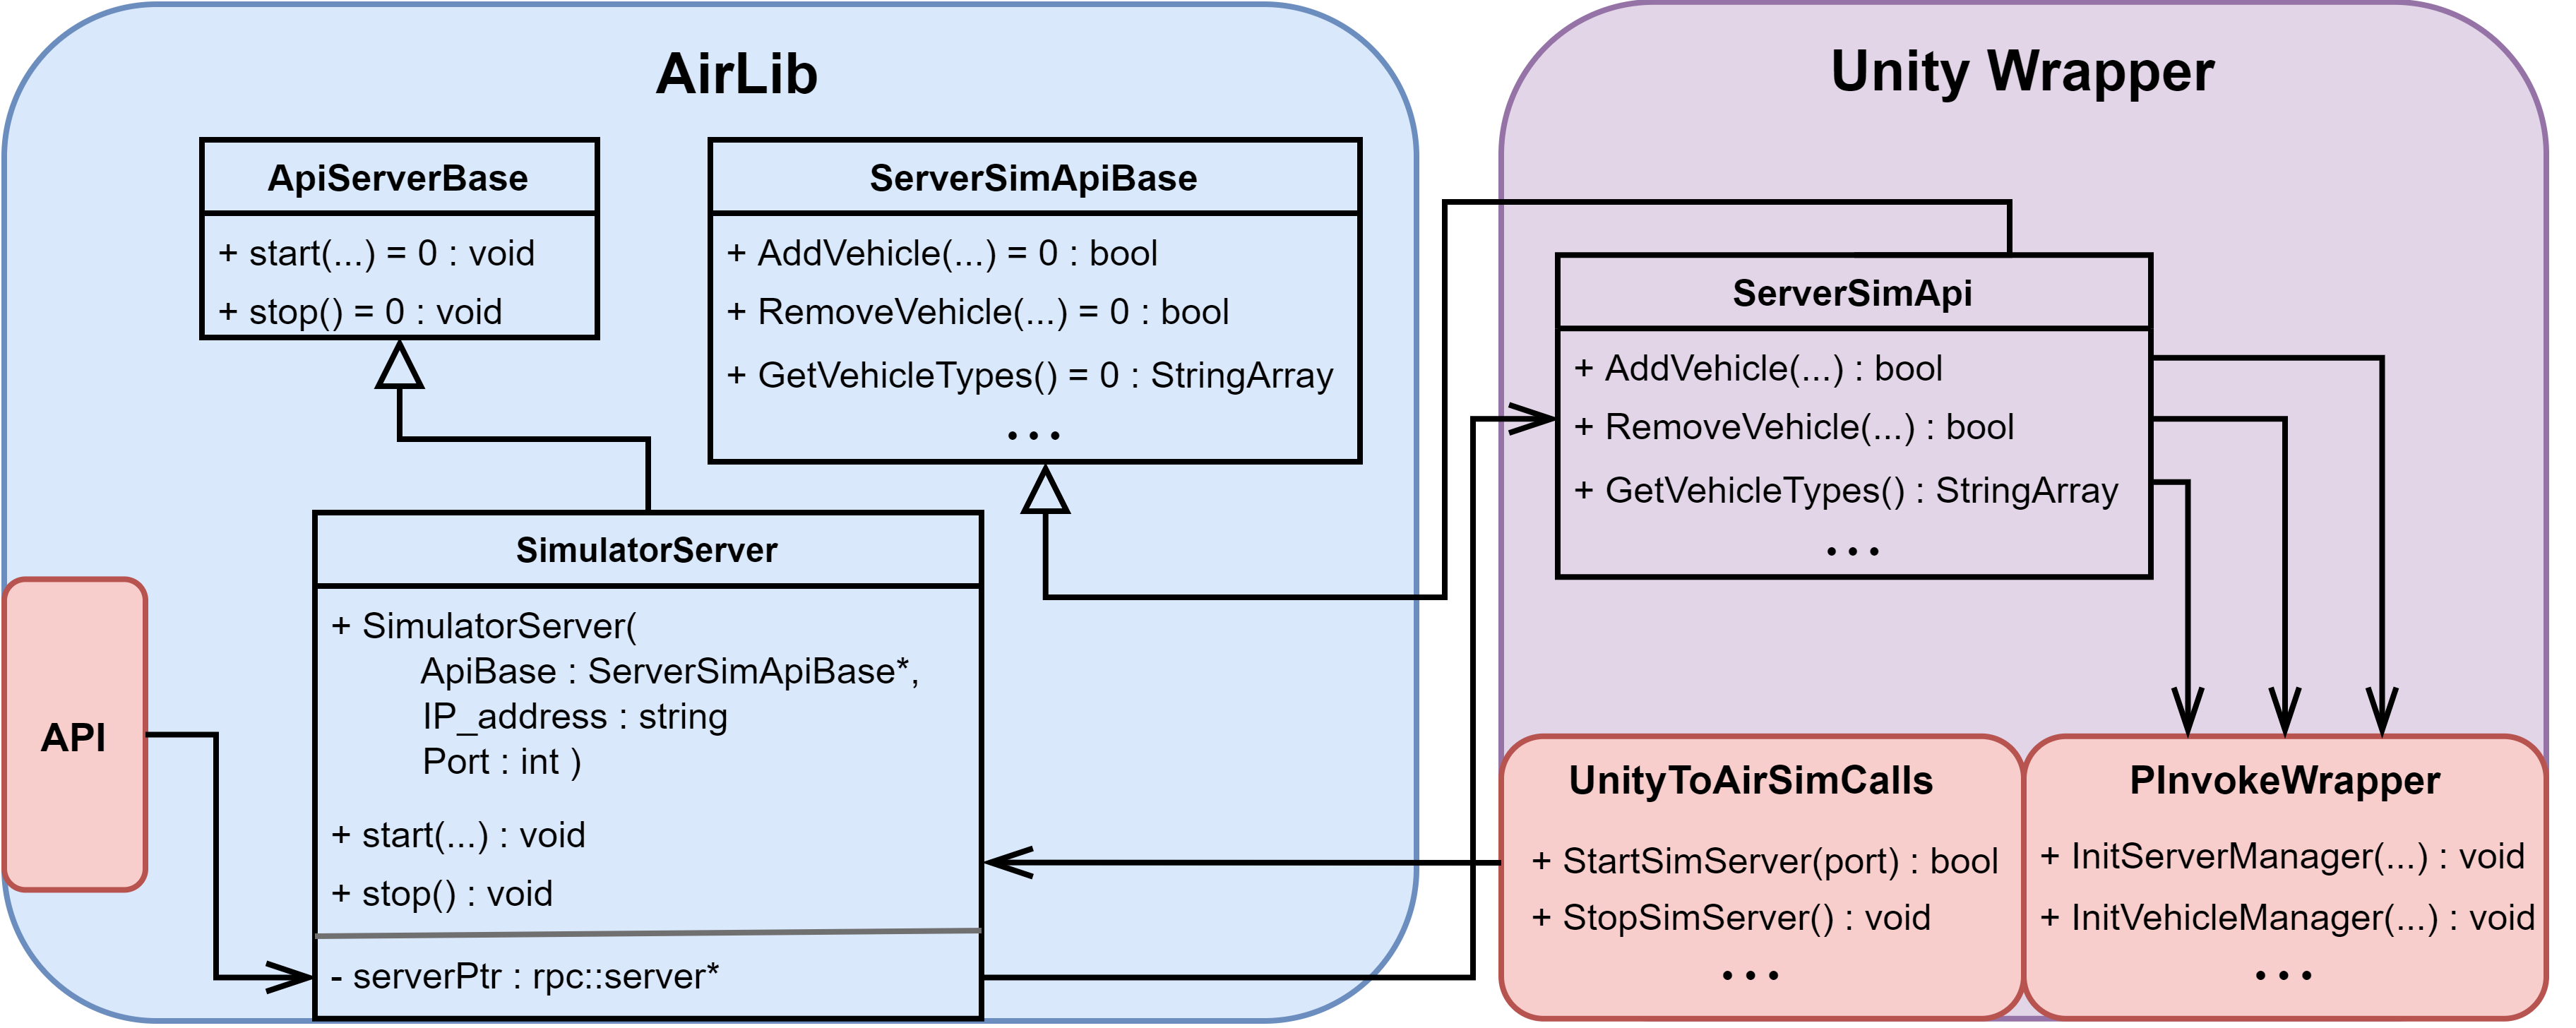
\includegraphics[width=1\textwidth]{05_AnalysisAndDesign/Diagrams/UnityWrapper2.png}
    \caption{A simplified view of how AirLib and the Unity Wrapper link together}
\end{figure}

\section{Architectural Design}
% Modularity
\paragraph{Dividing the server}
\paragraph{Moving logic to Unity}
\paragraph{Simplifications}
\section{Architectural Limitations}

